\subsection{Photo Measures}

\subsubsection{Vorstellung}
Die App \pm{} von \emph{Big Blue Pixel Inc.} hat zur Zeit des Downloads (30. November 2017, Version \emph{1.3.0}) bei insgesamt 1 461 abgegeben Bewertungen eine durchschnittliche Bewertung von 3,7 von 5 Sternen im Google Play-Store\urlnote{https://play.google.com/store/apps/details?id=com.bigbluepixel.photomeasures.lite}{30.11.2017}.
Auch diese App wird im Play-Store unter der Kategorie ``Effizienz'' gelistet.
Zu den in der App-Beschreibung aufgelisteten positiven Rezensionen von verschiedensten Webseiten und Magazinen, schreibt der Entwickler selbst noch folgende Wort \citep{PixelPM}:

\begin{quote}
  ``Photo Measures is the best and easiest way to save measures on your own photos on Android.
  [...] Whenever you need to save dimensions, sizes, angles or write down a detail you need to remember, Photo Measures will help you to be more efficient and more accurate.''
\end{quote}

\noindent
Beim initialen Start der App wird ein \emph{Tooltip} über der Statusleiste angezeigt (siehe \autoref{fig:pmmenu}).
Dieser \emph{Tooltip} zeigt auf ein Plus-Icon in der Statusleiste und gibt zusätzlich noch einen kurzen erklärenden Text zu der Aktion, die sich hinter diesem Icon verbirgt.

\begin{figure}[h]
  \begin{subfigure}[t]{0.3\textwidth}
    \centering
    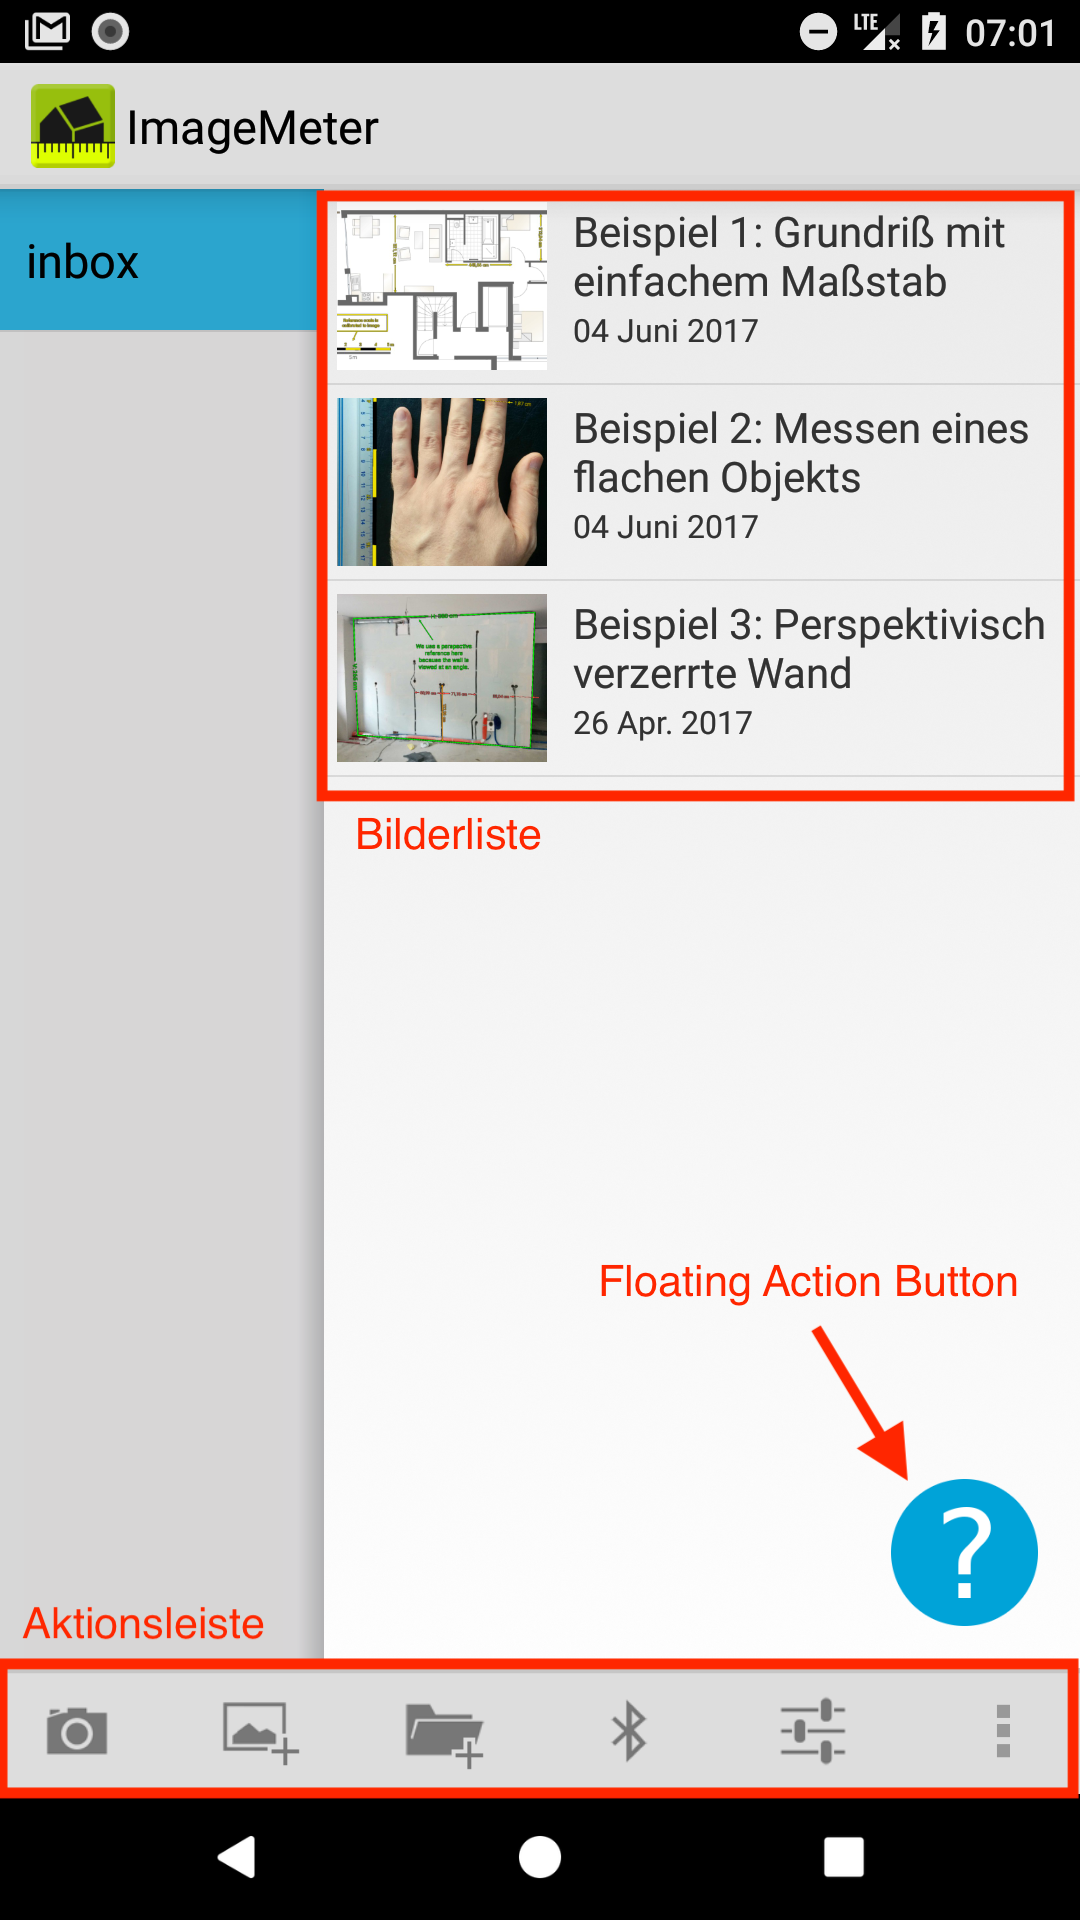
\includegraphics[keepaspectratio, width=\textwidth]{photo_measures/menu}
    \caption{Startbildschirm}
    \label{fig:pmmenu}	
  \end{subfigure}
  ~
  \begin{subfigure}[t]{0.3\textwidth}
    \centering
    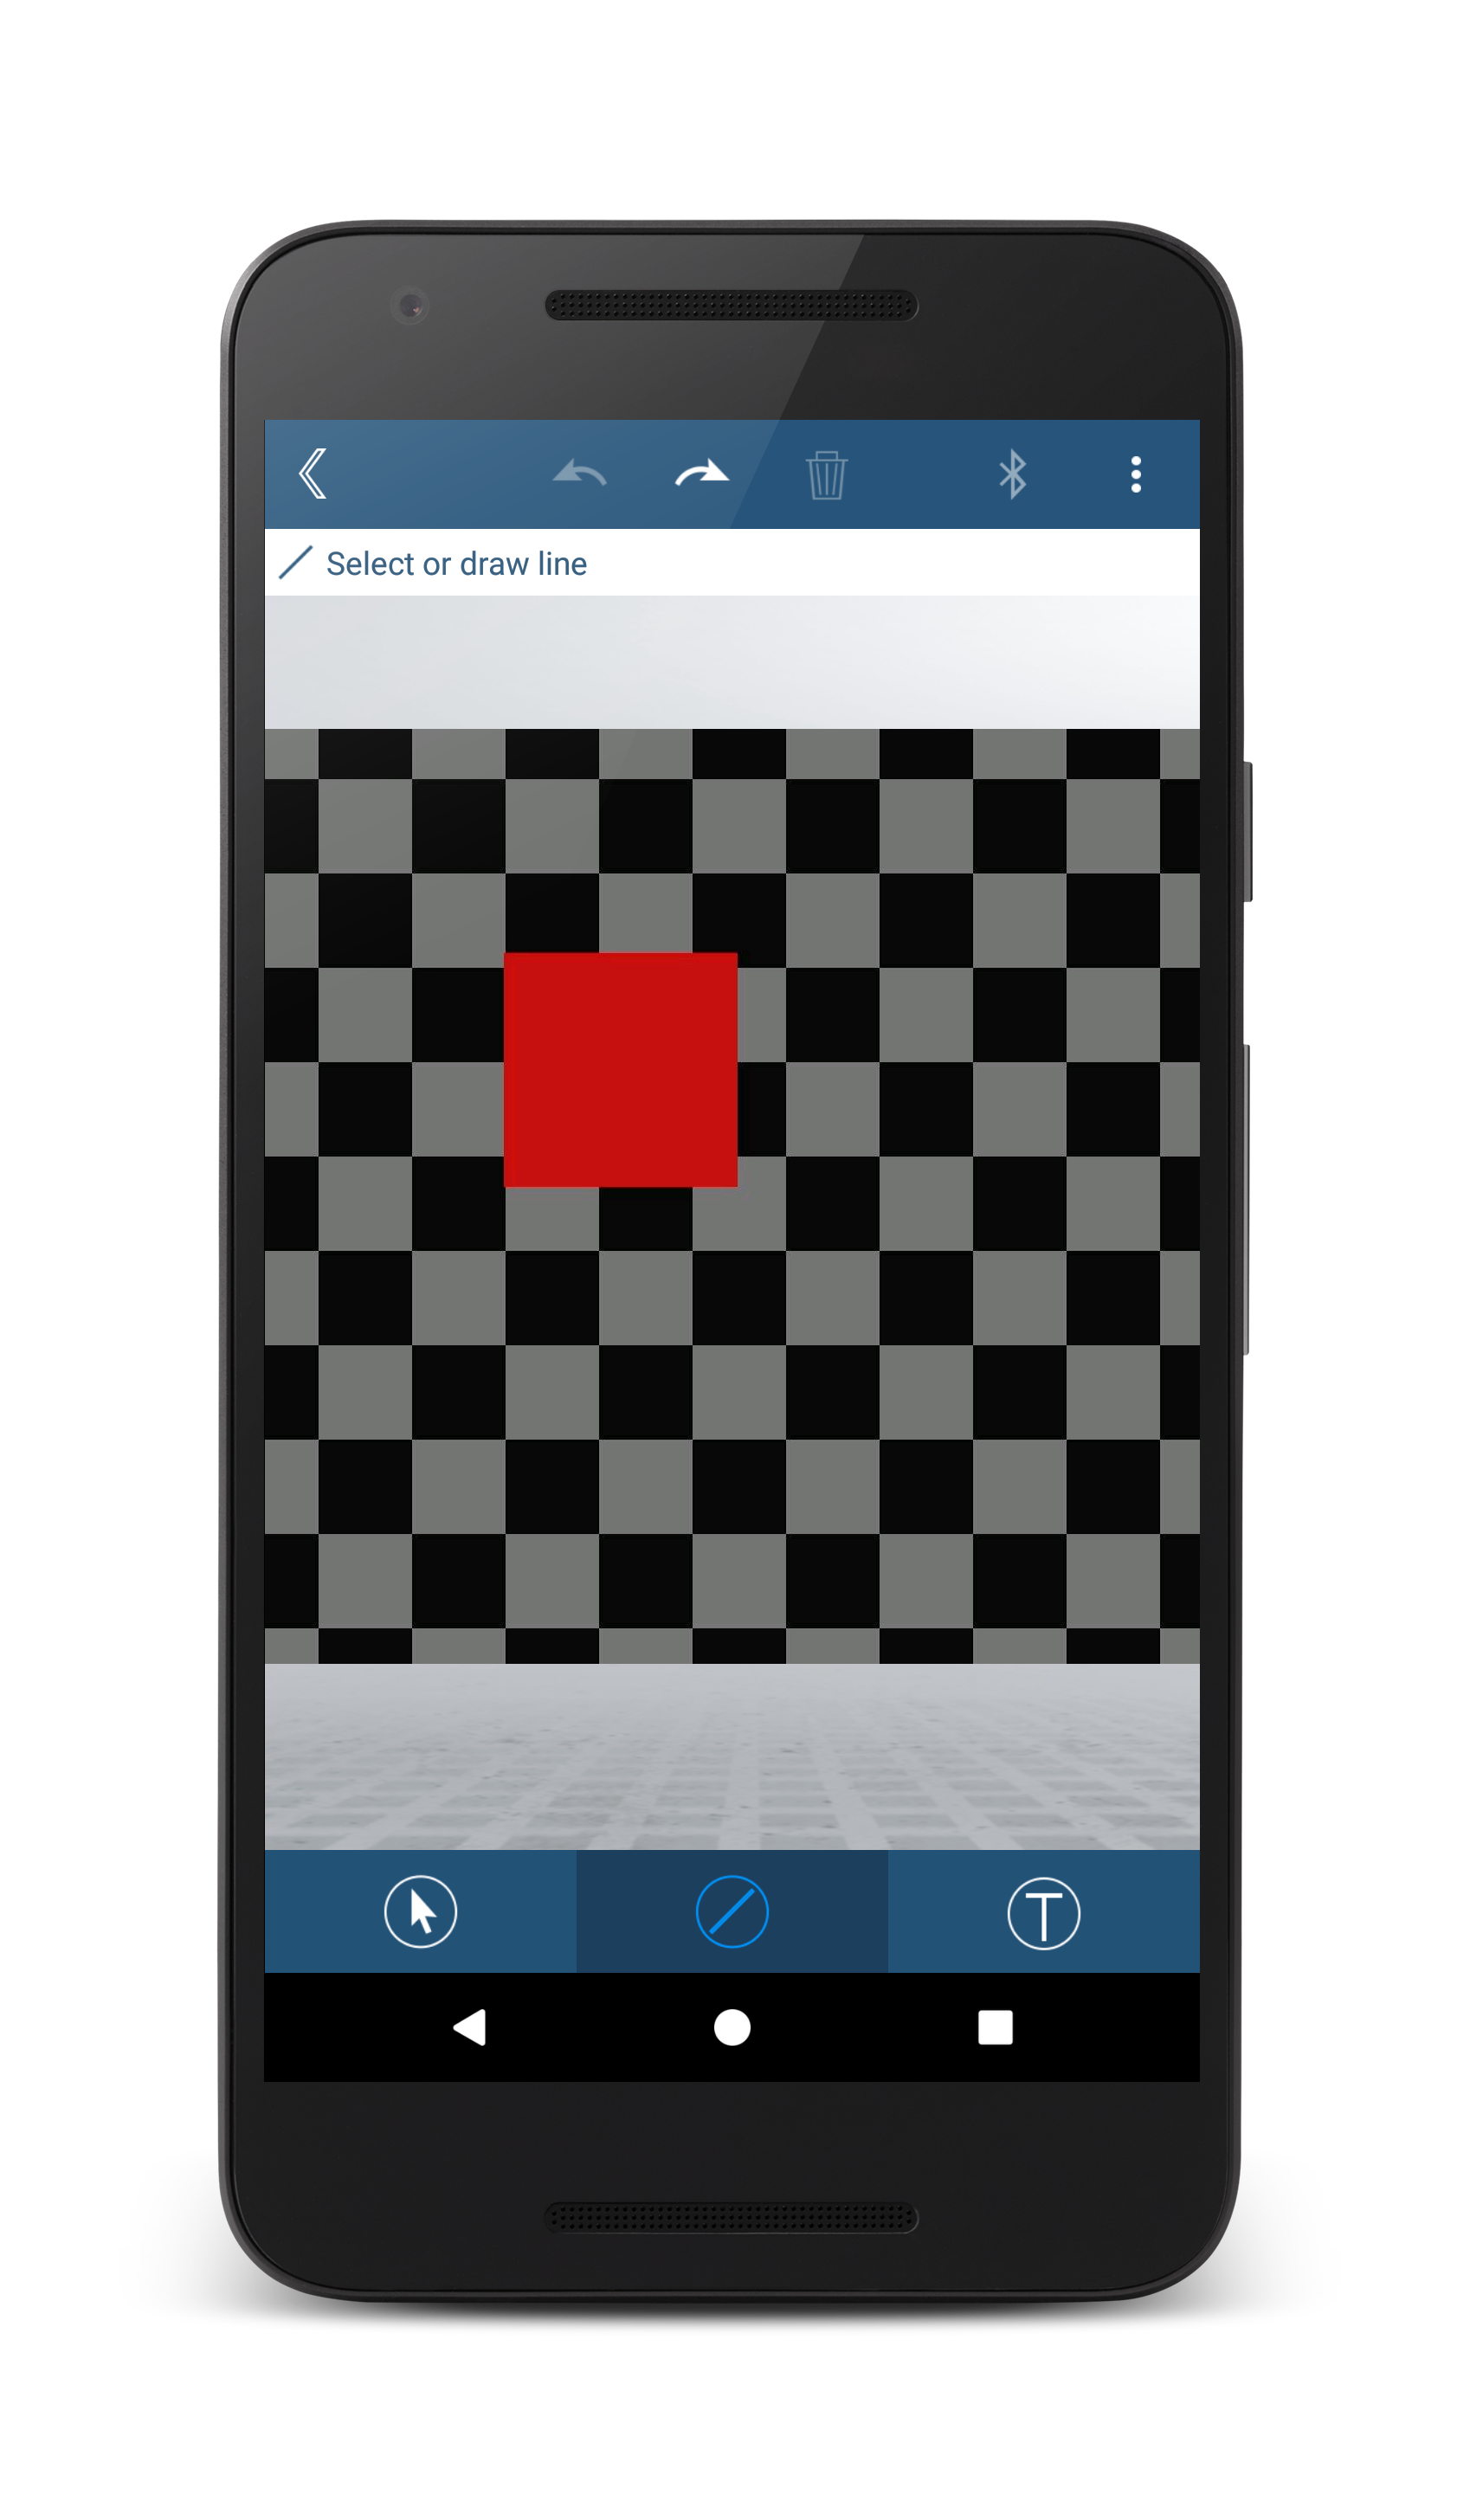
\includegraphics[keepaspectratio, width=\textwidth]{photo_measures/help}
    \caption{Hilfe-Overlay beim initialen Start der Aufmaß-Funktion} 
    \label{fig:pmhelp}	
  \end{subfigure}
  ~
  \begin{subfigure}[t]{0.3\textwidth}
    \centering
    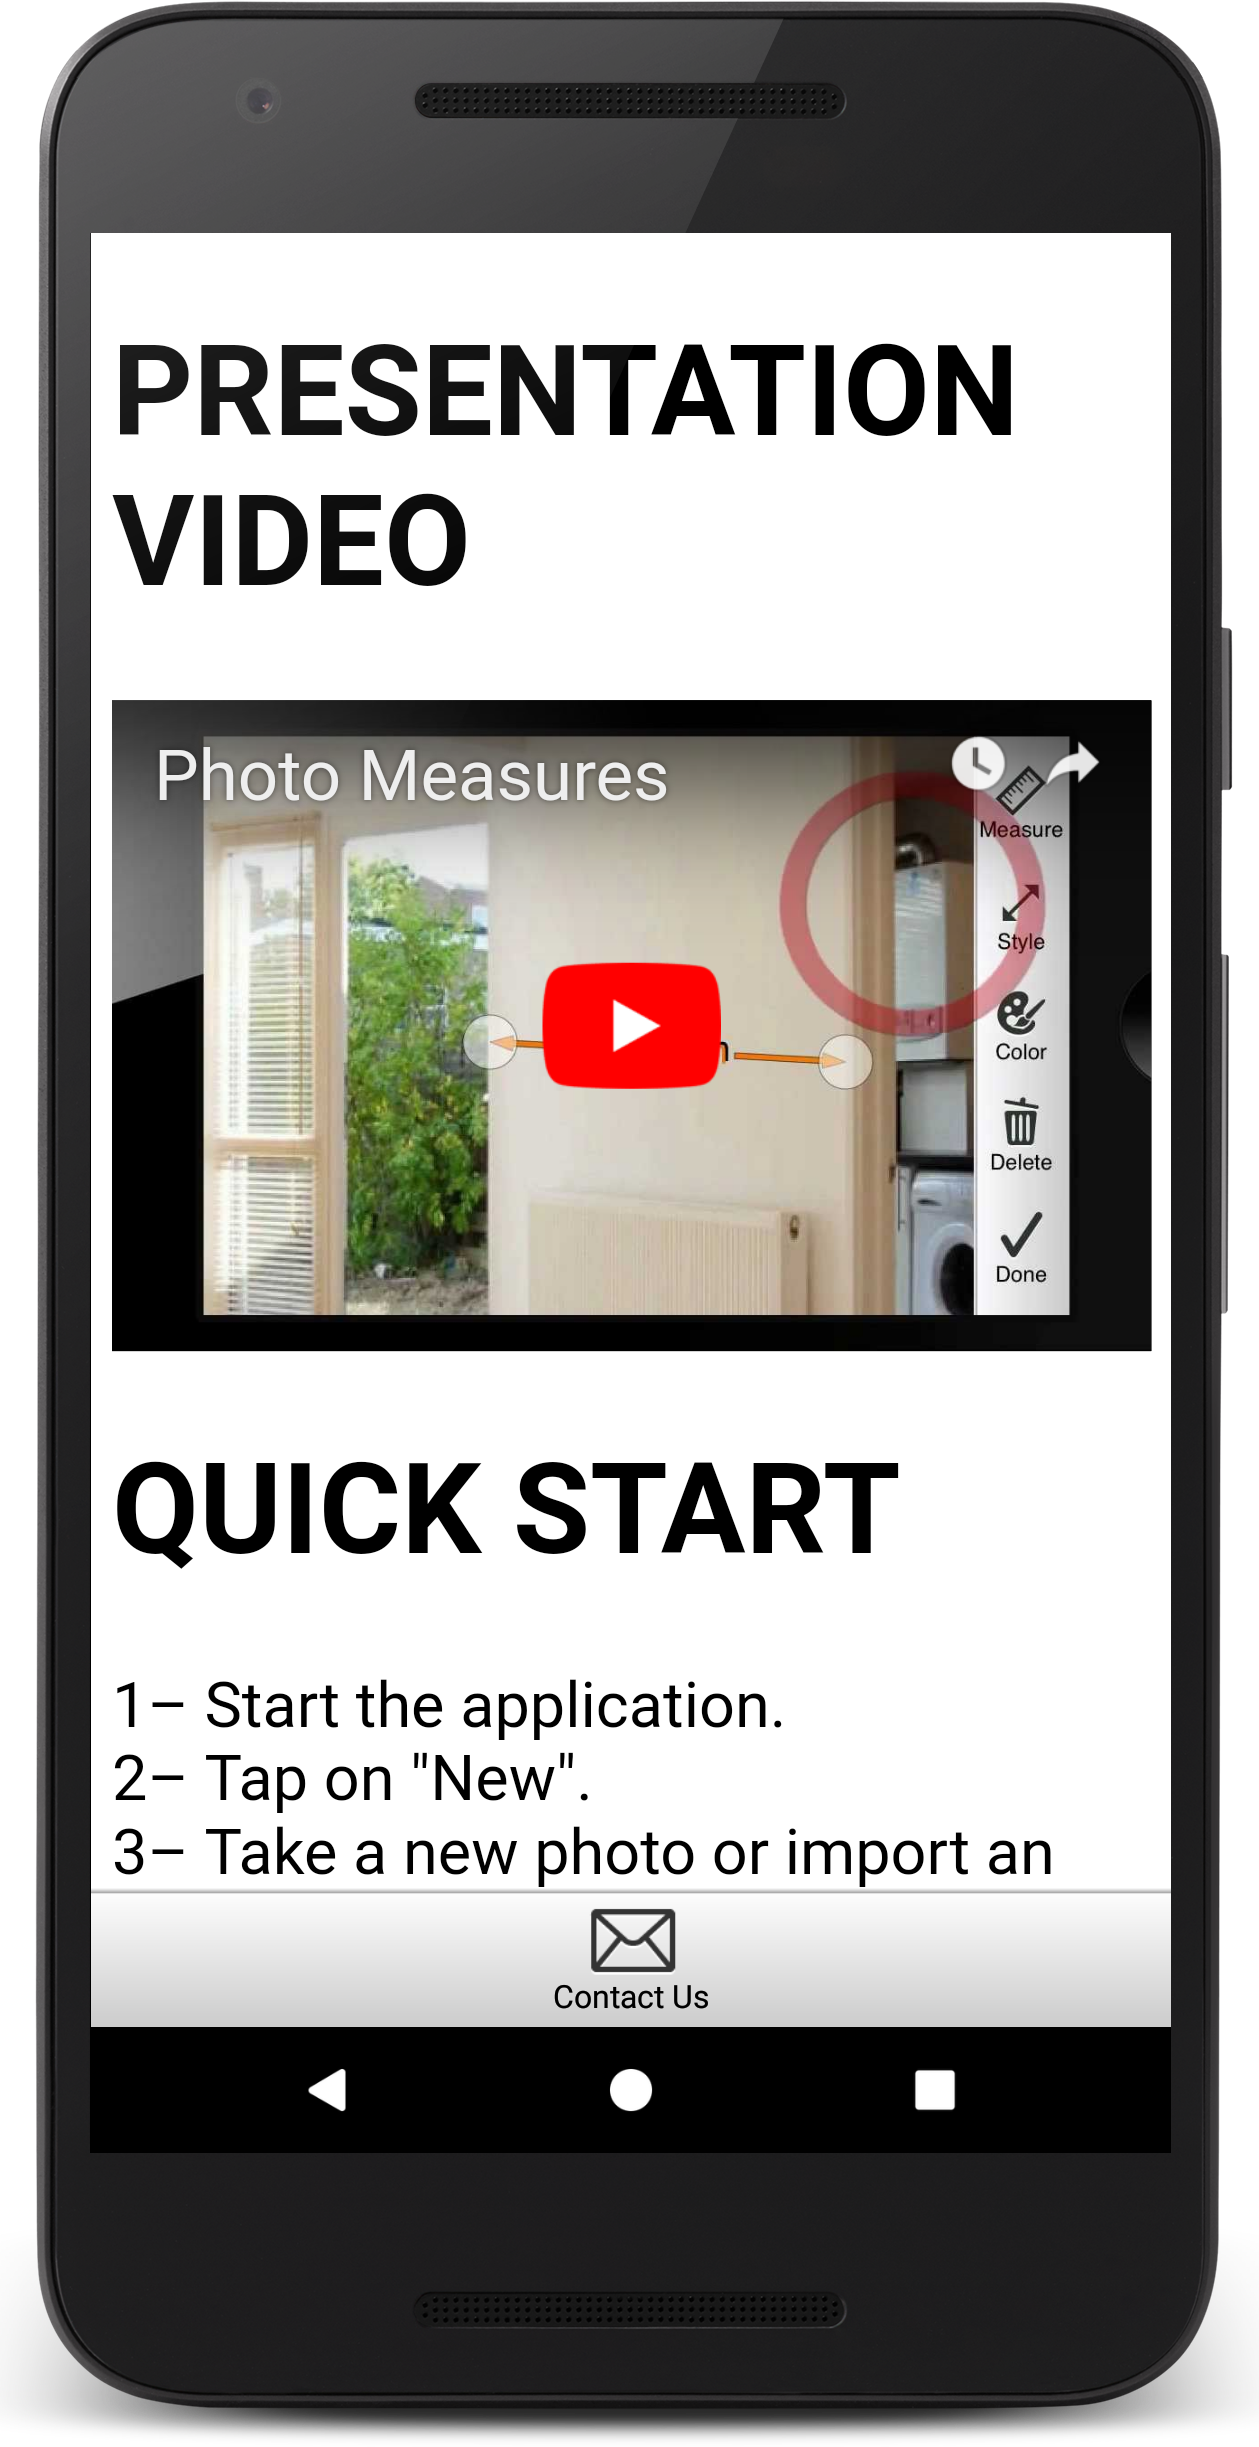
\includegraphics[keepaspectratio, width=\textwidth]{photo_measures/qs}
    \caption{\emph{Quick-Start Guide}}
    \label{fig:pmqs}
  \end{subfigure}
  \centering
  \caption{\pm{} beim Start der App und in der Aufmaß-Funktion}
\end{figure}

\noindent
Durch einen Klick auf das beschriebene Plus-Icon öffnet sich ein Dialog, der den Benutzer auffordert, ein Bild auszuwählen.
Hierzu kann der Benutzer direkt ein Bild aus der Galerie importieren, oder ein Neues mit der Kamera aufnehmen. \\

Anschließend wechselt die App in eine andere Benutzeroberfläche.
Hier werden die zuvor angezeigten Icons der Statusleiste durch vier neue Icons ersetzt und das ausgewählte Bild angezeigt (siehe \autoref{fig:pmhelp}).
Wenn der Benutzer diese Oberfläche zum ersten Mal öffnet, zeigt die App außerdem ein Hilfe-Overlay.
Dieses stellt die drei möglichen Gesten zur Navigation in der Oberfläche jeweils mit Hilfe eines Icons und kurzen Satzes dar. 
Sobald der Nutzer den Bildschirm berührt, wird das Hilfe-Overlay ausgeblendet. \\

Die Statusleiste bietet dem Benutzer nur die Funktionen an, die im aktuellen Systemzustand ausführbar sind.
Dies wird in dieser App so umgesetzt, dass eine weitere Statusleiste über die vorhandene geschoben wird, wenn eine Form markiert wird.
Diese eingeschobene Statusleiste bietet nur Aktionen zur Bearbeitung der markierte Form an und verdeckt somit gleichzeitig alle Aktionen, die im aktuellen Systemzustand nicht ausführbar seien sollen.
So hat der Nutzer, wenn keine Form markiert ist, die Möglichkeit zwischen drei verschiedenen Formen (Linie, Winkel, Freitext) zu wählen, die gewünschte Größe einzustellen, oder das Bild schrittweise um $90$ Grad im Uhrzeigersinn zu rotieren.
Außerdem kann in diesem Zustand über das Fragezeichen-Icon jederzeit ein \emph{Quick-Start Guide} aufgerufen werden (siehe \autoref{fig:pmqs}).
Wenn eine Form markiert ist, kann diese über die eingeschobene Statusleiste (siehe \autoref{fig:pmbar}) im Nachhinein beschriftet, in ihrer Zeichenart verändert, gefärbt oder gelöscht werden.
Sobald der Nutzer die Markierung aufhebt, wird die Statusleiste wieder ausgeblendet. \\

Auch in dieser App lassen sich bearbeitete Bilder speichern, und zu einem späteren Zeitpunkt weiter bearbeiten.
Zusätzlich ermöglicht die App das Exportieren mehrerer Bilder in einer \emph{PDF} oder jeweils als einzelnes \emph{JPG}.

\subsubsection{Evaluation}\label{subsec:pmeva}
Das initiale Hilfe-Overlay, welches beim Wechsel in die Bearbeitungs-Oberfläche angezeigt wird dient zusammen mit dem \emph{Quick-Start Guide} als Hilfe und Dokumentation der App (Nielsen \autoref{itm:N10}).
Besonders die Benutzung von Schaubildern im Hilfe-Overlay (\autoref{fig:pmhelp}) gestalten die initiale Benutzung der App intuitiv und einfach. \\

Fehleranfällige Situationen werden durch die Benutzung einer jeweils dedizierten Statusleiste präventiv vermieden (Nielsen \autoref{itm:N5}).
Hier kann der Nutzer im jeweiligen Systemzustand nur die Aktionen durchführen, die von der aktuell sichtbaren Statusleiste angeboten werden.
Zusätzlich zur präventiven Fehlervorbeugung sorgt dies für eine angemessene und verständliche Rückmeldung über den derzeitigen Systemzustand der App (Nielsen \autoref{itm:N1}). \\

\begin{wrapfigure}{R}{0.4\textwidth}
  \centering
  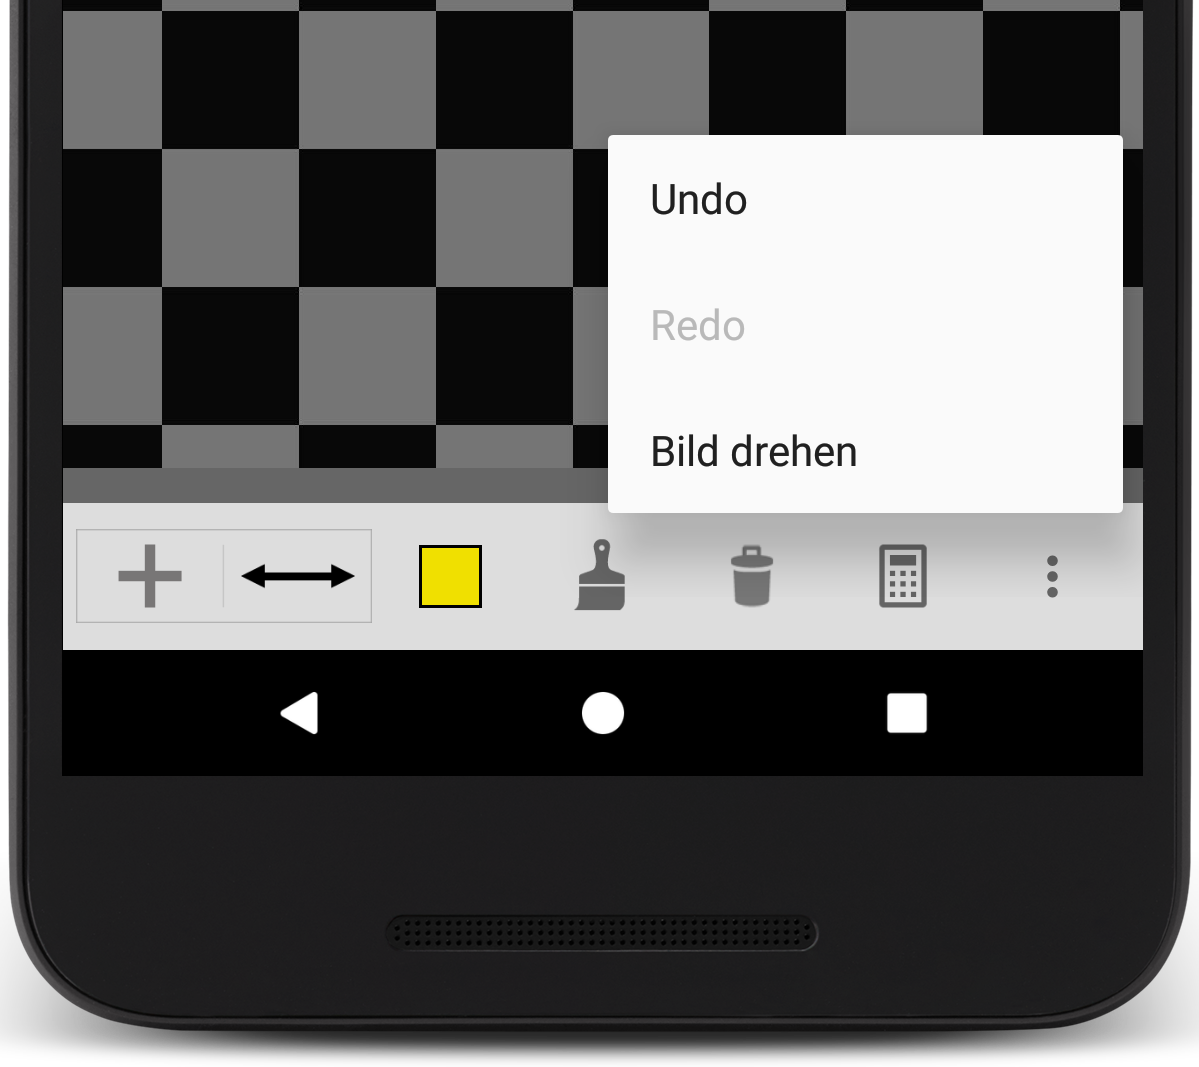
\includegraphics[keepaspectratio, width=0.4\textwidth]{photo_measures/bar}
  \caption{Statusleiste bei ausgewählter Form}
  \label{fig:pmbar}
\end{wrapfigure}

\noindent
Die App bedient sich einer Reihe bekannter Icons, sodass intuitiv erkennbar ist, welche Aktion sich hinter welchem Icon in der Statusleiste verbirgt (Nielsen~\autoref{itm:N6} \& \autoref{itm:N4}).
Wird ein Icon dennoch nicht erkannt, so stehen zusätzlich die Aktionen in Textform unter diesen (siehe \autoref{fig:pmbar}). \\

Der Nutzer hat die Möglichkeit vor dem Zeichnen der Formen, die Form- sowie Text-Größe einzustellen.
Die ausgewählte Zeichenfarbe wird für alle weiteren Formen übernommen, sodass diese nur ein einziges Mal konfiguriert werden muss.
Dies sorgt nicht nur eine flexible und individuelle, sondern auch für eine effizientere Benutzung der App, da diese nur einmal zu Beginn wie gewünscht konfiguriert werden muss (Nielsen~\autoref{itm:N7}). \\

Im Gegensatz dazu steht die fehlende Benutzerkontrolle (Nielsen \autoref{itm:N3}) der App.
So ist es dem Benutzer nicht möglich, über einen Undo- bzw. Redo-Button seine Aktionen rückgängig zu machen bzw. zu wiederholen.
Dies ist gerade bei der Bearbeitung von Bildern, bei welcher es viele aufeinander aufbauende Aktionen des Benutzers gibt, eine essentielle Funktionalität, die fehlt.
Hierdurch wird einerseits das Nutzungserlebnis negativ beeinflusst, da fehlerhafte Eingaben vollständig gelöscht, und anschließend neu ausgeführt werden müssen (Nielsen~\autoref{itm:N13}).
Andererseits wirkt sich eine fehlende Undo- bzw. Redo-Funktion auch negativ auf die kognitive Last des Benutzers aus.
Dieser muss sich alle ausgeführten Bearbeitungsschritte für den Fall einer fehlerhaften Eingabe merken, um diese anschließend erneut ausführen zu können (Nielsen~\autoref{itm:N9}). \\

Besonders auffällig wird die fehlende Benutzerkontrolle in Kombination mit der fehlerhaften \emph{Pinch-Geste} zum Zoomen des Bildes.
Hierbei zeichnet der Nutzer beim Ausführen der \emph{Pinch-Geste} ungewollt eine Form auf das Bild (Nielsen \autoref{itm:N16}).
Da die App keinerlei Möglichkeit bietet, unabsichtlich ausgeführte Aktionen rückgängig zu machen, muss der Nutzer nach jeder Zoom-Aktion die eingezeichnete Form löschen und kann erst danach mit der eigentlichen Bearbeitung der App fortfahren.
Gerade bei der Bearbeitung von Bilder mit vielen Details ist die Navigation im Bild und insbesondere das Zoomen unausweichlich. \\

Ein positiver Aspekt dagegen liegt in der Unterstützung der verschiedenen Bildschirmausrichtungen, sowie dem adäquaten Umgang mit Unterbrechungen.
Der Nutzer kann die App jederzeit drehen, ohne dass Informationen in der App verloren gehen oder der Benutzer durch eine unerwartete Neuausrichtung des Bildes verwirrt wird (Nielsen \autoref{itm:N11} \& \autoref{itm:N15}). \\

\begin{wrapfigure}{R}{0.4\textwidth}
  \centering
  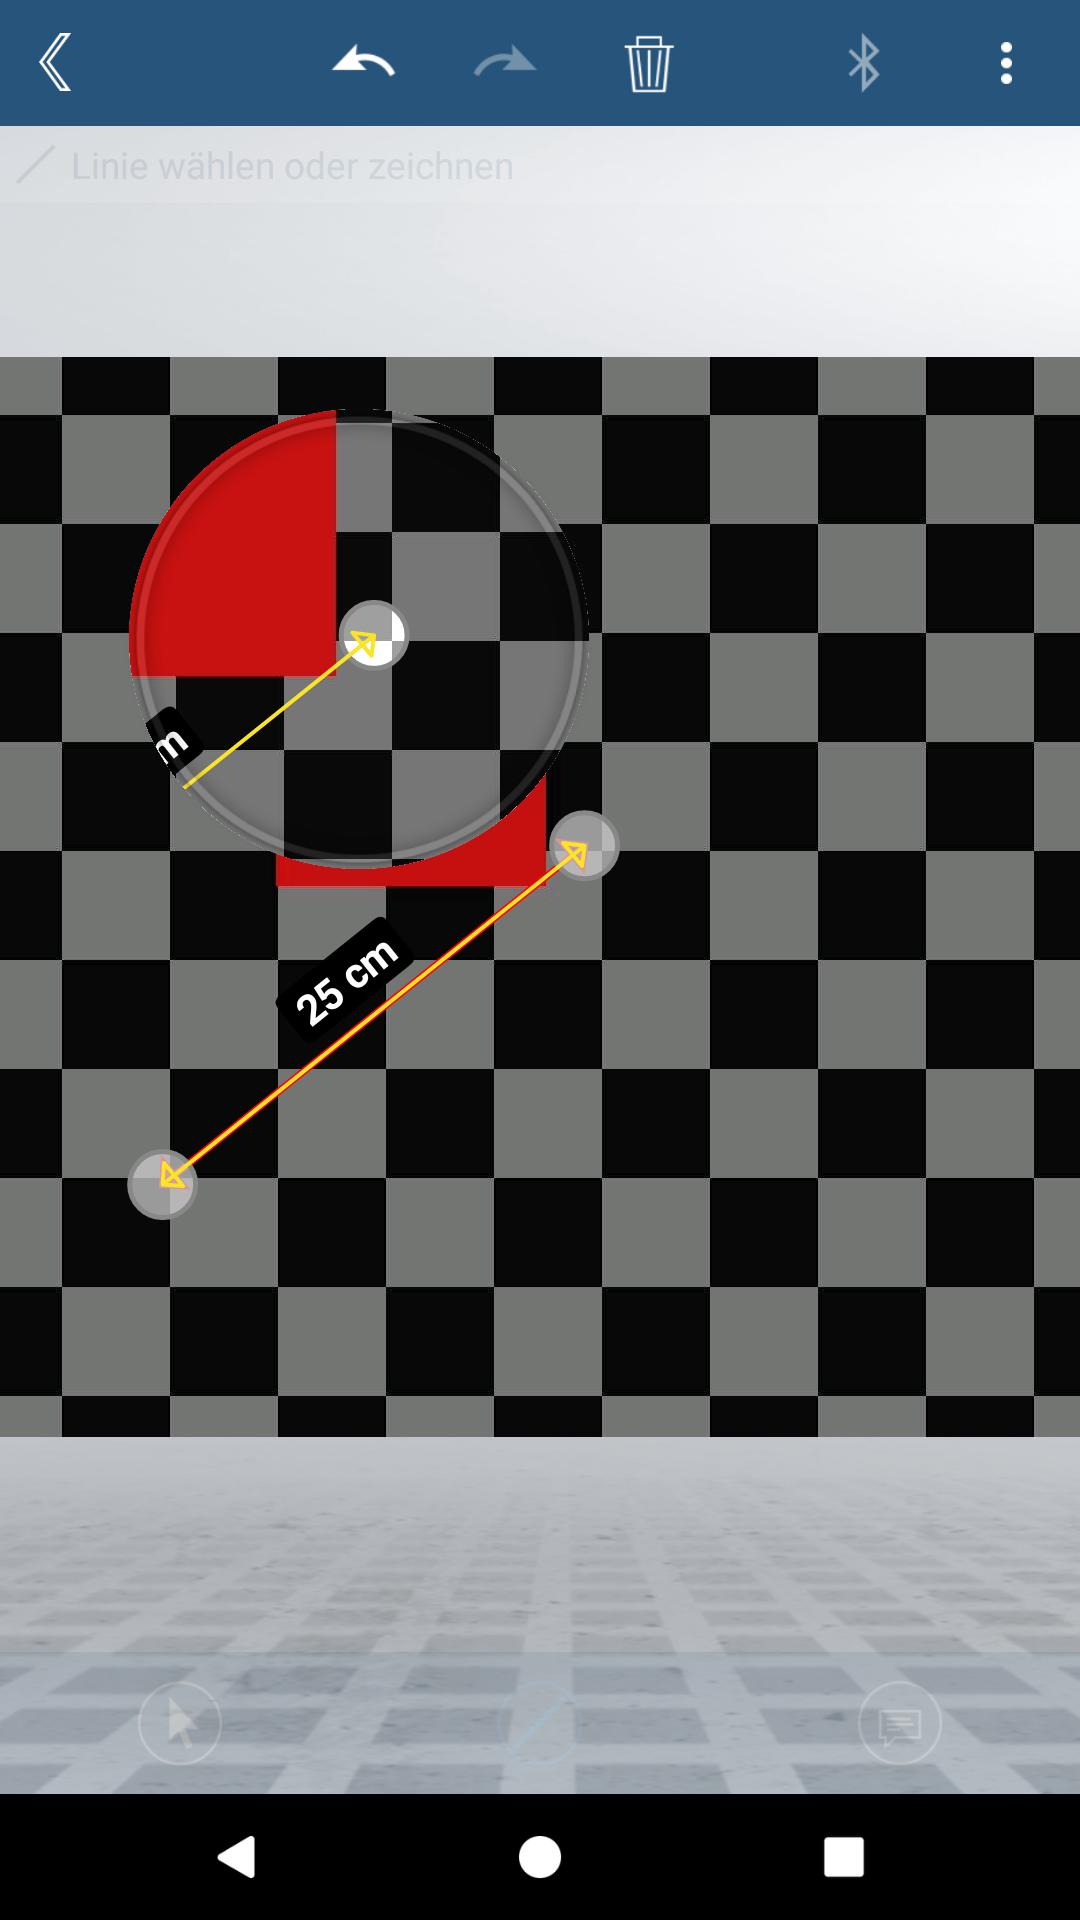
\includegraphics[keepaspectratio, width=0.4\textwidth]{photo_measures/lense}
  \caption{Zoom-Linse beim Zeichnen einer Linien-Form}
  \label{fig:pmlense}
\end{wrapfigure}

Die einfache Handhabung und das Zeichnen von Formen mit einem Finger ermöglichen eine einhändige Benutzung der App (Nielsen~\autoref{itm:N17}).
Zudem benutzt auch diese App eine Zoom-Linse, um den Bereich, der beim Zeichnen vom Finger verdeckt wird, an einer anderen Stelle vergrößert darzustellen (siehe \autoref{fig:pmlense}).
Dies beugt Fehlern beim Zeichnen der Formen vor und erhöht außerdem die Effizienz, da der Nutzer nicht jedes Mal erst den Finger vom Bildschirm nehmen muss, um zu sehen, bis wohin er die Form schon gezeichnet hat. \\

Eingetragene Messwerte stehen nach dem Exportieren der bearbeiteten Bilder nicht mehr als Meta-Daten zur Verfügung.
Hierdurch können die in der App annotierte Bilder nicht für die Weiterverarbeitung in einem nachgeschalteten Dienst genutzt werden (\autoref{itm:export}).
Außerdem lassen sich Bilder aus einer bestehenden App nicht in \pm{} teilen, sodass eine Integration in eine bestehende Systemarchitektur nur sehr mühsam möglich wäre (\autoref{itm:integration}). \\

Zusammenfassend kann also festgehalten werden, dass die App \pm{} von \emph{Big Blue Pixel} die Usability-Heuristiken nach Nielsen nur bedingt gut umsetzt, da besonders die Kombination der fehlerhaften \emph{Pinch-Geste} beim Zoomen mit der fehlenden Undo- bzw. Redo-Funktionalität zu einem negativen Anwendungserlebnis führen.
Der Benutzer muss hier also nach fast jeder Zoom-Aktion eine Lösch-Aktion ausführen, um die unabsichtlich gezeichnete Form wieder zu löschen.
Hierdurch wird nicht nur das Nutzungserlebnis geschmälert, sondern auch eine effiziente Nutzung der App als Alternative zur analogen Aufmaßerfassung nahezu unmöglich.
